\documentclass{article}
\usepackage[utf8]{inputenc}

%GENERAL
\usepackage[a4paper, inner=2cm, outer=1cm, top=2cm, bottom=2cm]{geometry}

%
\usepackage{amsmath}
%Figures & refs
\usepackage{caption}
\captionsetup{justification=centering}
\usepackage[dvipsnames]{xcolor}
\DeclareCaptionFont{black}{\color{black}}
\usepackage{hyperref}
\usepackage{tabularx}
\usepackage{booktabs}
\usepackage{float}
\usepackage{graphicx, calc}
\usepackage{enumerate}
%
\newlength\myheight
\newlength\mydepth
\settototalheight\myheight{Xygp}
\settodepth\mydepth{Xygp}
\setlength\fboxsep{0pt}
\newcommand*\inlinegraphics[1]{%
    \settototalheight\myheight{Xygp}%
    \settodepth\mydepth{Xygp}%
    \raisebox{-\mydepth}{\includegraphics[height=1.5\myheight]{#1}}%
}

%TIKZ
\usepackage{tikz}
\usetikzlibrary{shadows}
\usetikzlibrary{shapes}
\usetikzlibrary{positioning}
\usetikzlibrary{arrows}
%CODE
\captionsetup[lstlisting]{labelfont=black,textfont=black}
\DeclareCaptionType{algorithm}[Algorithm][List of algorithms]
\usepackage{listings}     
\usepackage{lstautogobble}  % Fix relative indenting
\usepackage{zi4}            % Nice font

\definecolor{keywords}{rgb}{0.93, 0.0, 0.71}
\definecolor{comments}{rgb}{0.6, 0.44, 0.80}
\definecolor{types}{rgb}{0.11, .1, 1.0}
\definecolor{numbers}{rgb}{0.6, 0.48, 0.78}
\definecolor{background}{rgb}{0.9, 0.9, 0.9}
\definecolor{foreground}{rgb}{0., 0., 0.}
\definecolor{strings}{rgb}{0.5, 0.0, 0.5}

\usepackage{listings}
\lstset{
    language=c++,
    autogobble,
    columns=fullflexible,
    showspaces=false,
    showtabs=false,
    breaklines=true,
    showstringspaces=false,
    breakatwhitespace=true,
    escapeinside={(*@}{@*)},
    emph={int, int32_t, float, double, unsigned, void, bool, char},
    emphstyle={\color{types}},
    backgroundcolor=\color{background},
    commentstyle=\color{comments},
    keywordstyle=\color{keywords},
    stringstyle=\color{strings},
    numberstyle=\color{numbers},
    basicstyle=\linespread{1.1}\ttfamily\color{foreground},
    frame=lbtr,
    framesep=0.1cm,
    xleftmargin=0.0cm,
    tabsize=4,
    captionpos=b
}
\renewcommand{\lstlistingname}{Code}
\newcommand{\tus}{\textunderscore}
\newcommand{\codet}[1]{\textcolor{black}{\textbf{\texttt{#1}}}}
\newcommand{\blt}[1]{\textcolor{blue}{#1}}

%NOTIONS AND WARNINGS
\newcommand{\Note}[1]{\vspace{0.5cm}\textcolor{blue}{NOTE: }{#1}\vspace{0.5cm}}
\newcommand{\Warning}[1]{\vspace{0.5cm}\textcolor{red}{WARNING: }{#1}\vspace{0.5cm}}


\title{Graphical User Interface for generation of CAEN WaveDump configuration file}
\author{LRDPRDX}
\date{\today}

%%%%%%%%%%%%%%%%%%%%%BEGIN%%%%%%%%%%%%%%%%%%%%%%
\begin{document}

\maketitle
\tableofcontents

\newpage
\section{Introduction}
This is a graphical user interface for generation of configuration files for the CAEN
WaveDump software. For now, it contains ONLY the configuration options that are
available for all the CAEN digitizers (particularly because I am able to test it on the
N6720A board only). Also it doesn't contain the register's operations yet.

\section{Installation}
To use it you need the following to be installed on your system
\begin{itemize}
    \item \codet{Python 2.7.x} or \codet{Python >=3.5}
    \item Packages for \codet{Python}:
            \begin{itemize}
                \item \codet{Tkinter}
            \end{itemize}
\end{itemize} 
Most probably all of the above packages are already installed provided \codet{Python}
is installed on your system.

Provided you've unpacked this package into \codet{<package\tus dir}, change to the
\codet{<package\tus dir/src} directory. There you will find the file named \codet{caenccf}.
You may need to make it executable. In linux the following command does the work:
\begin{lstlisting}
> chmod +x caenccf
\end{lstlisting}
Now just run it
\begin{lstlisting}
> ./caenccf
\end{lstlisting}
If everything is OK you should see the following window on your screen:
\begin{figure}[H]
    \centering
    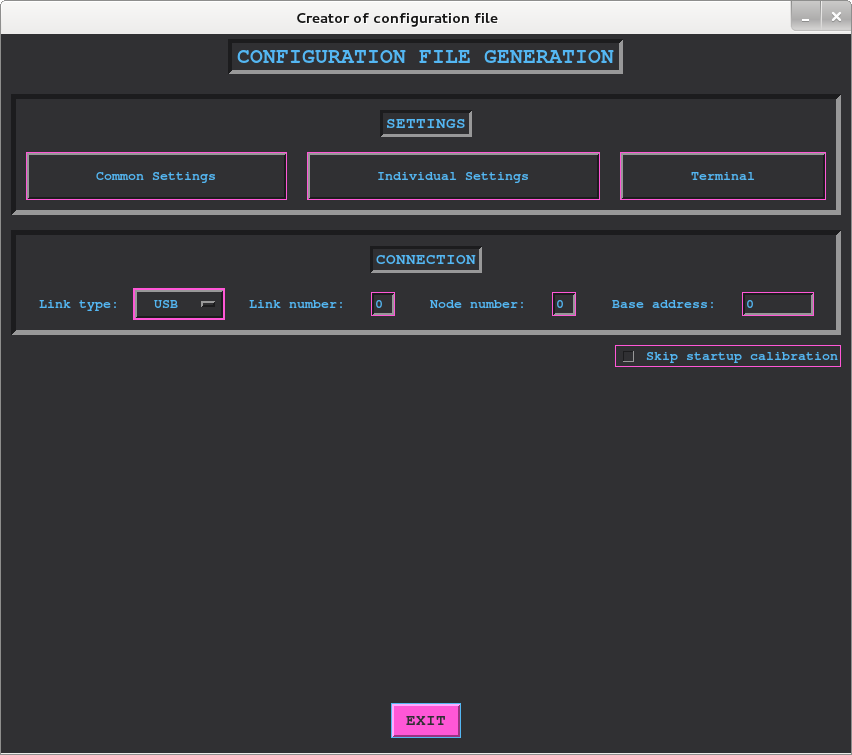
\includegraphics[width=0.8\textwidth]{../pictures/documentation/gui/start_page.png}
    \caption{GUI starting page}
    \label{fig:gui_stpg}
\end{figure}

It is very useful to be able to run it from everywhere on your system. In order to reach
this you need to place the executable in your \codet{bin} directory:
\begin{lstlisting}
> cp caenccf /usr/bin/
\end{lstlisting}
Also you need to extend the \codet{PYTHONPATH} environment variable in order \codet{Python}
to see necessary modules. Add the following lines in your \codet{.profile} (or \codet{.bash\tus profile}) file:
\begin{lstlisting}
if [[ -n "$PYTHONPATH" ]]; then
    PYTHONPATH=$PYTHONPATH:/path/to/<package_dir>/src
else
    export PYTHONPATH=/home/path/to/<package_dir>/src
fi;
\end{lstlisting}
Log out and log in back. After that you should be able to run the GUI from anywhere on your system. 

\section{Usage}
\subsection{Creating configuration file}
As it was mentioned in \textbf{Introduction} in order to configure a digitizer you must
use configuration file for \blt{WD}. The complete instruction how to create it see in
\blt{WD} documentation. This section is how to do this using the GUI presented in this
package. Here there will be no explanation of what each configure option means, for this,
please, check \blt{WD} documentation.

Firstly, open terminal and change to the directory when you want to place config-file.
Then run the GUI there:
\begin{lstlisting}
> caenccf
\end{lstlisting}
You will see the GUI's starting page (see~Fig.\ref{fig:gui_stpg}).
All configure options have the same names as in the official \blt{WD} documentation so
using is straightforward. However, some things require additional explanation. 
\subsubsection*{Pages}
The GUI consists of four pages (including the starting page). The \codet{Common Settings}
page contains configure options applied to each channel. The \codet{Individual Settings}
page is for the channels' configuration. The \codet{Terminal} settings contains terminal
frame for running \blt{WD} (see below).
\subsubsection*{Path to file}
It is possible to place config-file in a directory that differs from that in which the
GUI was launched. To save config-file wherever you wish use the \codet{Save to} entry

\begin{figure}[H]
    \centering
    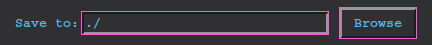
\includegraphics[width=0.4\textwidth]{../pictures/documentation/gui/path.png}
\end{figure}

By default it is the current directory (\codet{./}) but it can be changed either by
changing the entry directly or by using file browser: \codet{Browse} \inlinegraphics{../pictures/documentation/gui/browser.png} button.

\subsubsection*{Baseline and DC offset}
\begin{figure}[H]
    \centering
    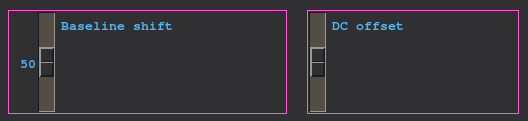
\includegraphics[width=0.4\textwidth]{../pictures/documentation/gui/baseline.png}
\end{figure}
As it is said in \blt{WD} documentation the \codet{BASELINE\tus SHIFT} and
\codet{DC\tus OFFSET} options \emph{are intended to be used one alternatively to the other}.
The GUI reflects this in the following way. If \codet{Use DC offset} \inlinegraphics{../pictures/documentation/gui/check.png} button is OFF then only \codet{Baseline shift} scale matters. Using
\codet{DC offset} scale has no effect. And vice-versa --- if that button is ON only
\codet{DC offset} scale is taken into account.

\subsubsection*{Trigger source option}
There are two choices for trigger: \codet{External} and \codet{Channel}. It seems that
\codet{External} trigger has higher priority for the acquisition. I.e. if you want to
use \codet{Channel trigger} for data acquisition you should choose the corresponding option
in the \codet{Channel trigger} option-menu:
\begin{figure}[H]
    \centering
    
\includegraphics[width=0.4\textwidth]{../pictures/documentation/gui/chan.png}
\end{figure}
\noindent AND disable external trigger in the \codet{External trigger} option-menu:
\begin{figure}[H]
    \centering
    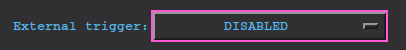
\includegraphics[width=0.4\textwidth]{../pictures/documentation/gui/ext.png}
\end{figure}

\subsubsection*{Saving configuration file} 

Once the configuration is done press \codet{Save} \inlinegraphics{../pictures/documentation/gui/save_btn.png}
button (right lower corner). If succeeded you should see the following popup window
\begin{figure}[H]
    \centering
    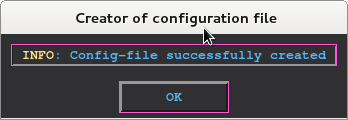
\includegraphics[width=0.4\textwidth]{../pictures/documentation/gui/success.png}
\end{figure} 
\noindent and a file called \codet{config.txt} inside the specified directory.

\subsubsection{Running WaveDump inside GUI}
After successful creation of a config-file it's time to run \blt{WD}.
In the \codet{Terminal} page one will find a frame with running \codet{xterm} inside.
It is intended to eliminate the need for users to use another window to run \blt{WD}.
Go to the \codet{Terminal} page and call \blt{WD} with the path to the config-file you
created before as an argument:
\begin{lstlisting}
> wavedump config.txt
\end{lstlisting}

\Warning{The terminal is running in the directory where the GUI was launched. And if you
chose another directory to save the config-file you must provide the full path to that file.
That is why it is recommended to run the GUI from the directory where you place a config-file.}

In the same page one will find \blt{WD} cheat sheet.  



\end{document}
